\documentclass[aspectratio=43]{beamer}

\usepackage[utf8]{inputenc}

\usepackage{amsfonts}
\usepackage{amsmath}
\usepackage{color}
\usepackage{listings}
\usepackage{tikz}
\usepackage{hyperref}

\usetheme{Rochester}
\usecolortheme{beaver}

\addtobeamertemplate{navigation symbols}{}{%
    \usebeamerfont{footline}%
    \usebeamercolor[fg]{footline}%
    \hspace{1em}%
    \insertframenumber/\inserttotalframenumber
}

\lstloadlanguages{C++}
    \lstset{%
        language={C++},
        basicstyle=\ttfamily,
        keywordstyle=\color{blue},
        showstringspaces=false,
        escapechar={§},
        escapeinside=||
    }

\newif\iftransitions
 \transitionstrue


\newif\iffast
% \fasttrue

\title{Taming Dynamic Memory}
\subtitle{An Introduction to Custom Allocators}
\author{Andreas Weis}
\institute{BMW AG}
\date{code::dive, November 7, 2018}
\titlegraphic{
\includegraphics[height=.2\textheight]{resources/codedive_logo.png}}

\iffalse
Taming dynamic memory - An introduction to custom allocators

Dynamic memory allocation is a feature that is often taken for granted. Most developers use some form of new or malloc every day, usually without worrying too much what goes on behind the scenes. But what about those situations where the built-in mechanisms are not good enough, be it for reasons of performance, safety, or due to restrictions of the target hardware? 

In this talk we will explore how custom allocators can be used to overcome those issues. We will explain how basic allocation techniques like pooling and monotonic allocation behave with regards to performance and reliability. We will take a look at some of the technical challenges behind allocators, like the different forms of alignment and the way that the standard library manages stateful allocators. And finally we will take a look at some popular allocator implementations and how to integrate them with a modern C++ codebase.

Audience
Developers that have never used a custom allocator before and don't know where to get started or don't understand what all the fuss is about.

Outline
- Scenarios in which the default allocator is not good enough
- Basic allocator toolbox: Stack, Monotonic, Pool, general-purpose; Explain the basic algorithm and pros & cons of each
- Popular open-source implementations of these
- Customization points for allocation in C++ and some popular third-party libraries; How they differ and how to bridge the gap.
- Using custom allocators for profiling, debugging and diagnostics
- Technical challenges when writing an allocator: Alignment, Strict aliasing, etc.
\fi

\begin{document}

\frame{\titlepage}

\iffalse %crop

\begin{frame}[fragile]
  \frametitle{About me}

  \begin{itemize}
    \setlength\itemsep{1.5em}

    \item \href{https://stackoverflow.com/users/577603/comicsansms}{
\includegraphics[height=.05\textheight]{resources/so-icon.png}} \href{https://github.com/ComicSansMS}{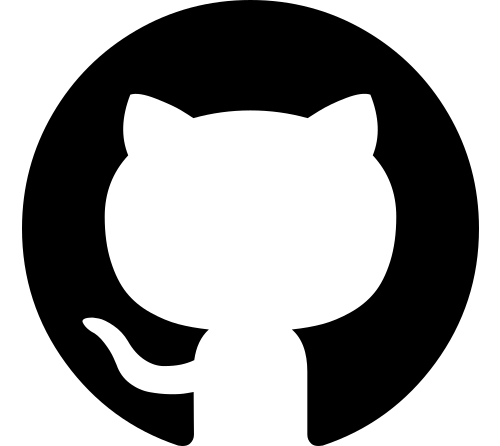
\includegraphics[height=.05\textheight]{resources/github-icon.png}} 
\includegraphics[height=.05\textheight]{resources/slack-icon.png} ComicSansMS

    \item \href{https://twitter.com/DerGhulbus/}{
\includegraphics[height=.05\textheight]{resources/twitter-icon.png} @DerGhulbus}

    \item 
\includegraphics[height=.05\textheight]{resources/meetup-icon.png} Co-organizer of the \href{https://www.meetup.com/MUCplusplus/}{Munich C++ User Group}

    \item Currently working as a Software Architect for BMW 
\includegraphics[height=.1\textheight]{resources/bmw_group.jpg}

  \end{itemize}
\end{frame}


\begin{frame}[fragile]
  \frametitle{General purpose allocator}
  \begin{center}
    \includegraphics<1>[width=.9\textwidth]{memgfx/gp_alloc_000.png}
    \includegraphics<2>[width=.9\textwidth]{memgfx/gp_alloc_010.png}
    \includegraphics<3>[width=.9\textwidth]{memgfx/gp_alloc_020.png}
%    \includegraphics<4>[width=.9\textwidth]{memgfx/gp_alloc_030.png}
    \includegraphics<4>[width=.9\textwidth]{memgfx/gp_alloc_040.png}
  \end{center}

    \begin{semiverbatim}
      \uncover<2->{\alert<0>{{\color{blue}auto} p1 = allocate(3);}}
      \uncover<3->{\alert<0>{{\color{blue}auto} p2 = allocate(4);}}
      \uncover<4->{\alert<0>{{\color{blue}auto} p3 = allocate(1);}}
      \uncover<4->{\alert<0>{{\color{blue}auto} p4 = allocate(3);}}
      \uncover<4->{\alert<0>{{\color{blue}auto} p5 = allocate(2);}}
    \end{semiverbatim}
\end{frame}


\begin{frame}[fragile]
  \frametitle{General purpose allocator}
  \begin{center}
    \includegraphics<1-2>[width=.9\textwidth]{memgfx/gp_alloc_040.png}
    \includegraphics<3>[width=.9\textwidth]{memgfx/gp_alloc_050.png}
    \includegraphics<4>[width=.9\textwidth]{memgfx/gp_alloc_060.png}
  \end{center}

    \begin{semiverbatim}
      \uncover<2->{\alert<2>{deallocate(p2);}}
      \uncover<4->{\alert<0>{{\color{blue}auto} p6 = allocate(2);}}
    \end{semiverbatim}
\end{frame}


\begin{frame}[fragile]
  \frametitle{Fragmentation}
  \begin{center}
    \includegraphics<1->[width=.9\textwidth]{memgfx/gp_alloc_060.png}
  \end{center}

    \begin{semiverbatim}
      \uncover<1->{\alert<0>{{\color{blue}auto} p7 = allocate(4);}}
      \uncover<2->{\alert<2>{\it{Runtime Error!}}}
    \end{semiverbatim}
\end{frame}


\begin{frame}[fragile]
  \frametitle{Coalescing}
  \begin{center}
    \includegraphics<1>[width=.9\textwidth]{memgfx/gp_alloc_060.png}
    \includegraphics<2-3>[width=.9\textwidth]{memgfx/gp_alloc_070.png}
    \includegraphics<4>[width=.9\textwidth]{memgfx/gp_alloc_080.png}
    \includegraphics<5>[width=.9\textwidth]{memgfx/gp_alloc_090.png}
  \end{center}

    \begin{semiverbatim}
      \uncover<1->{\alert<1>{deallocate(p4);}}
      \uncover<3->{\alert<3>{deallocate(p3);}}
    \end{semiverbatim}
\end{frame}


\begin{frame}[fragile]
  \frametitle{Monotonic Allocator}
  \begin{center}
    \includegraphics<1-2>[width=.9\textwidth]{memgfx/monot_010.png}
    \includegraphics<3>[width=.9\textwidth]{memgfx/monot_020.png}
    \includegraphics<4>[width=.9\textwidth]{memgfx/monot_030.png}
  \end{center}

  \begin{semiverbatim}
    \uncover<2->{\alert<2>{{\color{blue}auto} p1 = monot.allocate(3);}}
    \uncover<4->{\alert<2>{{\color{blue}auto} p2 = monot.allocate(2);}}
    \uncover<4->{\alert<2>{{\color{blue}auto} p3 = monot.allocate(4);}}
  \end{semiverbatim}
\end{frame}


\begin{frame}[fragile]
  \frametitle{Monotonic Allocator}
  \begin{center}
    \includegraphics<1>[width=.9\textwidth]{memgfx/monot_030.png}
    \includegraphics<2>[width=.9\textwidth]{memgfx/monot_040.png}
    \includegraphics<3>[width=.9\textwidth]{memgfx/monot_050.png}
    \includegraphics<4-5>[width=.9\textwidth]{memgfx/monot_060.png}
  \end{center}

  \begin{semiverbatim}
    \uncover<1->{\alert<1>{monot.deallocate(p2);}}
    \uncover<3->{\alert<3>{monot.deallocate(p1);}}
    \uncover<3->{\alert<3>{monot.deallocate(p3);}}
    
    \uncover<4->{\alert<4>{{\color{blue}auto} p4 = allocate(2);}}
  \end{semiverbatim}
\end{frame}


\begin{frame}[fragile]
  \frametitle{Monotonic Allocator - Reclamation}
  \begin{center}
    \includegraphics<1>[width=.9\textwidth]{memgfx/monot_060.png}
    \includegraphics<2-3>[width=.9\textwidth]{memgfx/monot_070.png}
    \includegraphics<4>[width=.9\textwidth]{memgfx/monot_010.png}
  \end{center}

  \begin{semiverbatim}
    \uncover<1->{\alert<1>{monot.deallocate(p4);}}

    \uncover<3->{\alert<3>{monot.release();}}
  \end{semiverbatim}
\end{frame}


\begin{frame}[fragile]
  \frametitle{Monotonic Allocator}
  \begin{itemize}
  \item Deterministic runtime cost
  \item Extremely efficient
  \item No fragmentation
  \item Easy to implement
  \item Trivial to make thread-safe
  \end{itemize}
  But:
  \begin{itemize}
  \item Memory can only be reclaimed all at once
  \end{itemize}
\end{frame}


 \begin{frame}[fragile]
  \frametitle{Monotonic Allocator - \texttt{std::vector}}
  \begin{center}
    \includegraphics<1>[width=.9\textwidth]{memgfx/monot_vector_010.png}
    \includegraphics<2>[width=.9\textwidth]{memgfx/monot_vector_020.png}
    \includegraphics<3>[width=.9\textwidth]{memgfx/monot_vector_030.png}
  \end{center}
\end{frame}


\begin{frame}[fragile]
  \frametitle{Monotonic Allocator - STL containers}
  \begin{itemize}
  \item \texttt{vector} should \texttt{reserve} final size upfront
  \item \texttt{list} and \texttt{map} work fine, but deleted elements are not reclaimed individually
  \item \texttt{unordered\_map} has same problem as \texttt{vector} when growing but the load-factor triggering rehash is less predictable
  \end{itemize}
\end{frame}


\begin{frame}[fragile]
  \frametitle{Monotonic Allocator - Extensions}
  \begin{itemize}
  \item Stack
  \item Stack Coalescing
  \item Queue
  \end{itemize}
\end{frame}


\begin{frame}[fragile]
  \frametitle{Pool Allocator}
  \begin{center}
    \includegraphics<1>[width=.9\textwidth]{memgfx/pool_010.png}
    \includegraphics<2-3>[width=.9\textwidth]{memgfx/pool_020.png}
    \includegraphics<4>[width=.9\textwidth]{memgfx/pool_030.png}
    \includegraphics<5-6>[width=.9\textwidth]{memgfx/pool_040.png}
  \end{center}

  \begin{semiverbatim}
    \uncover<2->{\alert<2>{{\color{blue}auto} p1 = pool.allocate(2);}}
    \uncover<2->{\alert<2>{{\color{blue}auto} p2 = pool.allocate(4);}}
    \uncover<2->{\alert<2>{{\color{blue}auto} p3 = pool.allocate(3);}}
    
    \uncover<4->{\alert<4>{pool.deallocate(p1);}}
    \uncover<5->{\alert<5>{{\color{blue}auto} p4 = pool.allocate(1);}}
  \end{semiverbatim}
\end{frame}


\begin{frame}[fragile]
  \frametitle{Pool Allocator - Reclamation}
  \begin{center}
    \includegraphics<1>[width=.9\textwidth]{memgfx/pool_free_010.png}
    \includegraphics<2-3>[width=.9\textwidth]{memgfx/pool_free_020.png}
    \includegraphics<4>[width=.9\textwidth]{memgfx/pool_free_030.png}
    \includegraphics<5-6>[width=.9\textwidth]{memgfx/pool_free_040.png}
  \end{center}

  \begin{semiverbatim}
    \uncover<2->{\alert<2>{{\color{blue}auto} p1 = pool.allocate(2);}}
    \uncover<2->{\alert<2>{{\color{blue}auto} p2 = pool.allocate(4);}}
    
    \uncover<4->{\alert<4>{pool.deallocate(p1);}}
    \uncover<5->{\alert<5>{pool.deallocate(p2);}}
  \end{semiverbatim}
\end{frame}


\begin{frame}[fragile]
  \frametitle{Pool Allocator - Diffusion}
  \begin{center}
    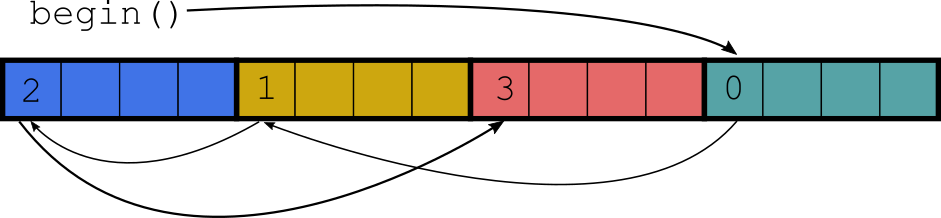
\includegraphics[width=.9\textwidth]{memgfx/pool_diffusion.png}
  \end{center}
\end{frame}


\begin{frame}[fragile]
  \frametitle{Multipool Allocator}
  \begin{center}
    \includegraphics<1-2>[width=.9\textwidth]{memgfx/multipool_010.png}
    \includegraphics<3-4>[width=.9\textwidth]{memgfx/multipool_020.png}
    \includegraphics<5>[width=.9\textwidth]{memgfx/multipool_030.png}
  \end{center}

  \begin{semiverbatim}
    \uncover<2->{\alert<2>{{\color{blue}auto} p1 = multipool.allocate(6);}}
    \uncover<4->{\alert<4>{{\color{blue}auto} p2 = multipool.allocate(2);}}
  \end{semiverbatim}
\end{frame}


\fi %crop


\begin{frame}[fragile]
  \frametitle{Stack Allocator}
  \begin{center}
    \includegraphics<1-2>[width=.9\textwidth]{memgfx/monot_030.png}
    \includegraphics<3>[width=.9\textwidth]{memgfx/monot_padding_010.png}
    \includegraphics<4>[width=.9\textwidth]{memgfx/monot_padding_011.png}
  \end{center}

  \begin{semiverbatim}
    \uncover<2->{\alert<2-3>{monot.deallocate(p3);}}
  \end{semiverbatim}
\end{frame}


\begin{frame}
  \frametitle{Stack Allocator}
  \begin{itemize}
  \item Strict FIFO-ordering of allocations and deallocations
  \item No way for the implementation to check whether the deallocation order is correct!
  \end{itemize}
\end{frame}


\begin{frame}[fragile]
  \frametitle{Stack Allocator}
  \begin{center}
    \includegraphics<1-2>[width=.9\textwidth]{memgfx/monot_padding_012.png}
    \includegraphics<3-4>[width=.9\textwidth]{memgfx/monot_padding_011.png}
  \end{center}

  \begin{semiverbatim}
    \uncover<1-2>{\alert<1>{monot.deallocate(p3);}}
    \uncover<2>{\alert<2>{p3 == top  \checkmark}}
    \uncover<4>{\alert<4>{top = ???}}
  \end{semiverbatim}
\end{frame}



\begin{frame}
  \frametitle{Stack Allocator}
  \begin{itemize}
  \item Strict FIFO-ordering of allocations and deallocations.
  \item No way for the implementation to check whether the deallocation order is correct!
    \pause
  \item Free-pointer is reset to the same pointer passed to the \texttt{deallocate} call
    \pause
  \item Padding bytes may be lost
  \end{itemize}
\end{frame}


\begin{frame}[fragile]
  \frametitle{Padding}
  \begin{center}
    \includegraphics<1>[width=.9\textwidth]{memgfx/monot_030.png}
    \includegraphics<2>[width=.9\textwidth]{memgfx/monot_padding_020.png}
  \end{center}
\end{frame}


\begin{frame}[fragile]
  \frametitle{Alignment}
  \begin{semiverbatim}
    0xdeadbeef =

   d    e    a    d    b    e    e    f
 1101 1110 1010 1101 1011 1110 1110 1111
  \end{semiverbatim}
\end{frame}


\begin{frame}[fragile]
  \frametitle{Alignment}
  \begin{semiverbatim}
    0xdeadbeef =

   d    e    a    d    b    e    e    {\color{red}f}
 1101 1110 1010 1101 1011 1110 1110 111{\color{red}1}
  \end{semiverbatim}

  No alignment (1-byte aligned).
\end{frame}

\begin{frame}[fragile]
  \frametitle{Alignment}
  \begin{semiverbatim}
    0xdeadbeef =

   d    e    a    d    b    e    e    {\color{red}c}
 1101 1110 1010 1101 1011 1110 1110 11{\color{red}00}
  \end{semiverbatim}

  4-byte aligned.
\end{frame}


\begin{frame}[fragile]
  \frametitle{Alignment}
  \begin{semiverbatim}
    0xdeadbeef =

   d    e    a    d    b    e    e    {\color{red}8}
 1101 1110 1010 1101 1011 1110 1110 1{\color{red}000}
  \end{semiverbatim}

  8-byte aligned.
\end{frame}


\begin{frame}[fragile]
  \frametitle{Alignment}

  \begin{itemize}
  \item Alignment refers to the least-significant bits of the object address being 0
  \item Alignment requirements are always specified in powers of 2
  \item Each C++ type has a \textit{natural} alignment requirement (typically \texttt{alignof(T) == sizeof(T)})
    \item This is why \texttt{struct}s sometimes insert padding bytes between members
  \end{itemize}
\end{frame}


\begin{frame}[fragile]
  \frametitle{Alignment}

  \begin{itemize}
  \item Default allocator typically returns addresses aligned to \texttt{alignof(max\_align\_t)}, which is big enough for all built-in types
  \item Users may \texttt{extend} the alignment requirement for custom data types using \texttt{alignas}
  \end{itemize}

  \begin{lstlisting}
void* allocate(std::size_t bytes,
               std::size_t alignment);
  \end{lstlisting}
\end{frame}



\iffalse
\begin{frame}[fragile]
  \frametitle{Let's talk about memory}
    \begin{itemize}
    \item Dynamic memory: Request objects using allocate, deallocate to give memory back
    \item Done! Or is it?
    \end{itemize}
    Problems with global allocator:
    \begin{itemize}
    \item No one-size fits all allocation strategy. Every allocator has an achilles heel.
    \item Global allocators don't parallelize well. Allocation/Deallocation typically requires acquiring a lock.
    \item Runtime performance of global allocators is unpredictable. Understanding runtime behaviour requires understanding the entire program
    \item Overhead of the allocation algorithm might not be acceptable on the target hardware.
    \end{itemize}
\end{frame}

\begin{frame}[fragile]
  \frametitle{Main concerns about dynamic memory}
    \begin{itemize}
    \item Maximum overall memory consumption.
    \item Runtime behavior.
    \item Fragmentation.
    \end{itemize}
\end{frame}

\begin{frame}[fragile]
  \frametitle{Local allocators to the rescue}
    Pro:
    \begin{itemize}
    \item 
    \end{itemize}

    Con:
    \begin{itemize}
    \item Allocating memory requires access to an allocator.
    \end{itemize}
\end{frame}
\fi

\begin{frame}
  \frametitle{Thanks for your attention.}
\end{frame}


\end{document}
